%!TEX root = ../prace.tex

\chapter{Úvod}

V době vzniku této práce jsou velice populární hry s otevřeným světem. Lákají hráče na obsáhlost světa a možnost nelineárního řešení problémů a herních úkolů. Her s otevřeným světem najdeme nepřeberné množství v různých herních žánrech. My se zaměříme na podmnožinu her, které kromě otevřeného světa nabízí také možnosti budování struktur a vyžadují od hráče netriviální styl hraní, který mu umožňuje ve hře přežít. Průmyslově se tyto hry často označují jako \textit{Sanboxové}, \textit{S budováním}, \textit{S průzkumem prostředí}, \textit{Survival}. Autor této práce má tento typ her v oblibě a rád by touto prací představil svoji vizi dalšího možného rozvoje her tohoto žánru. Cílem práce by měla být implementace nového herního principu stavění, které současné herní tituly nenabízí.

\section{Charakteristika her}
V práci se budeme zabývat několika různými hrami, které však mají několik společných vlastností. Jedním ze základních konceptů je využívání herních bloků. Dalším význačným prvkem je způsob integrace herních bloků do herního prostření. Některé hry jsou celé tvořeny bloky, jiné se snaží dosáhnout vyššího stupně realismu ve hře a bloky využívají pouze pro konstrukci různých herních objektů. Ústředním tématem této práce tedy bude rozbor systému bloků a práce s nimi a popis hráčských problémů způsobených danými koncepty. V další části práce pak navrhneme a implementujeme vlastní řešení.




\subsection{Hry kompletně blokové}
Začněme hrami, které využívají bloků jako základního elementu celé hry. Bloky zde tvoří doslova celý svět. Mezi nejpopulárnější a širokou veřejností nejznámější bychom měli zařadit hru \MC{}. Jak je zřejmé z obrázku \ref{fig:intro_mc}, celá hra včetně herní postavy, nehratelných postav - \gls{npc}, nebo třeba mraků, je stylizovaná do bloků ve tvaru kostky. Většina bloků je stejně velká a má hranu o délce 1 metru \citep{mc_block}, \citep{mc_units}. 

\begin{figure}[!ht]\centering
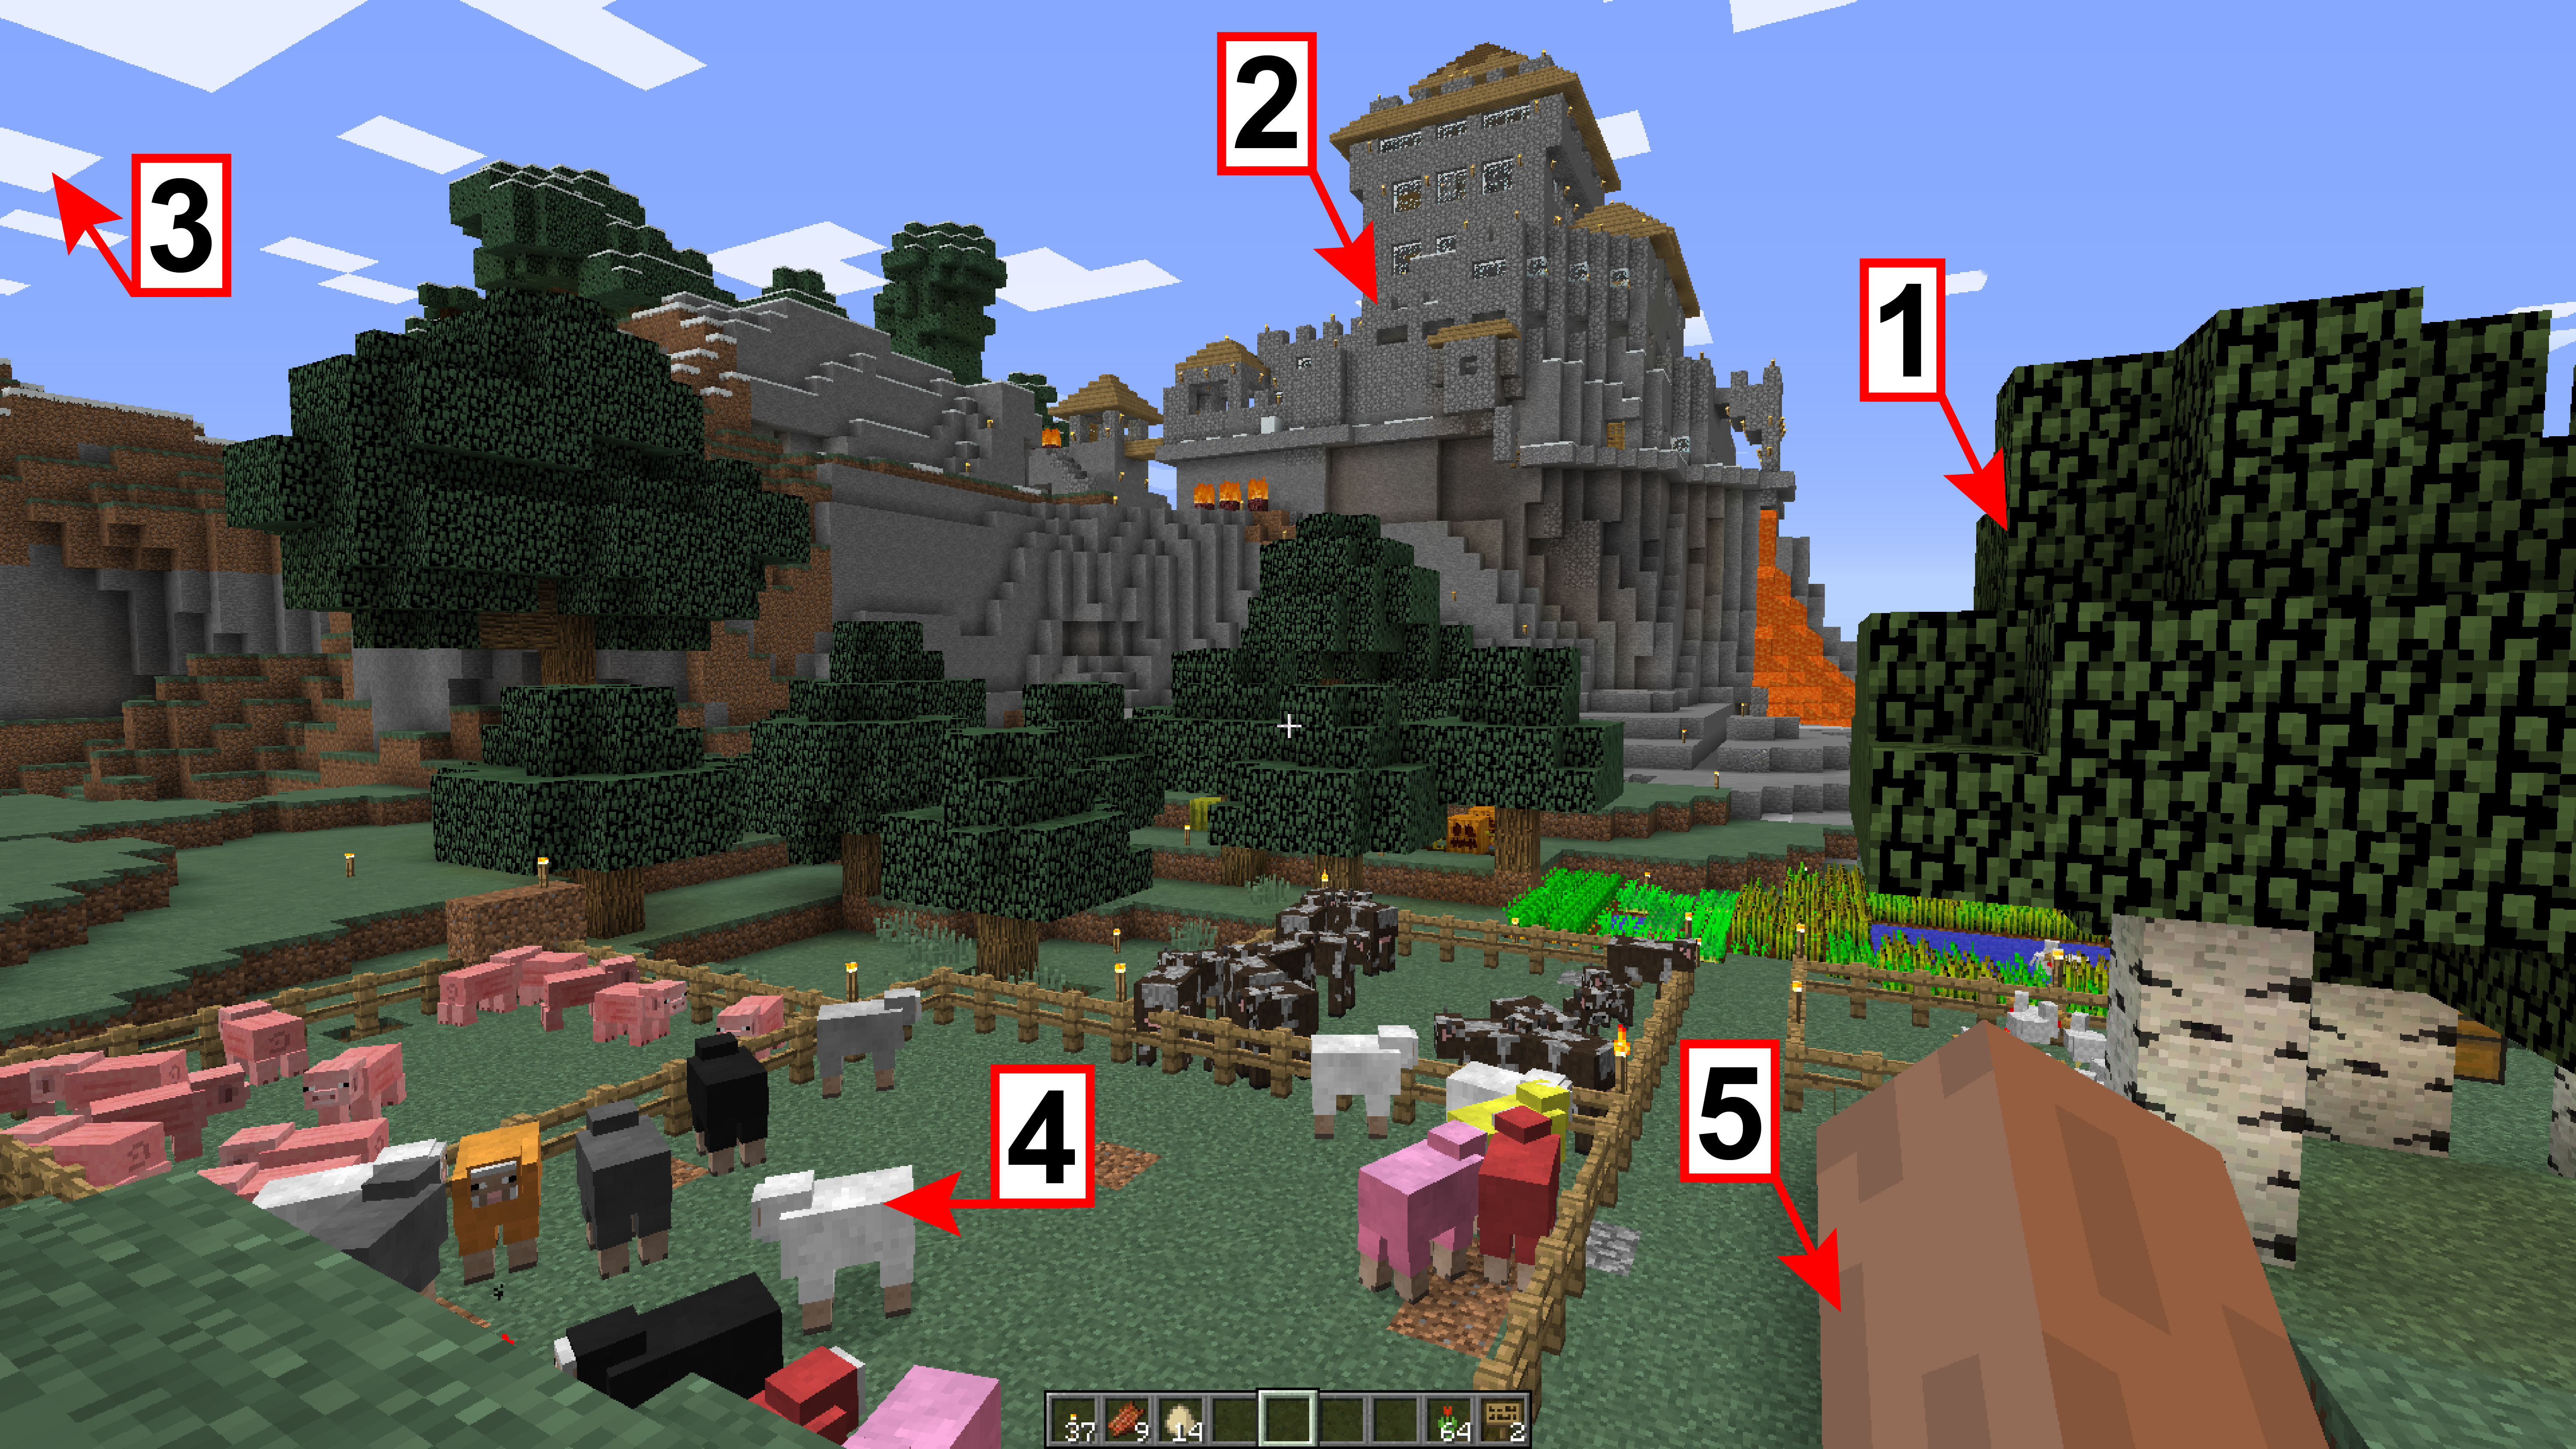
\includegraphics[ width=140mm]{../img/intro/mc}

\caption{Hra Minecraft - hrad na skále}
\label{fig:intro_mc}

\end{figure}

\FloatBarrier

Mezi dalšími hrami bychom mohli zmínit například \TE{}. Ta je o něco mladší než \MC{}, ale je častým zdrojem diskusí, zda je lepší new \MC{}, nebo ne. Pravdou je, že obě hry mají svůj svět kompletně složený z kostek (\TE{} je však 2D hra), ale každá si klade trochu jiné cíle. \TE{} je více orientovaná na příběh, obsahuje více NPC i bossů, \MC{} je orientován spíše na stavění. (Porovnání \citep{mc_te_comparsion})


\subsection{Hry s prvky realismu}

Mezi tyto hry bychom mohli zařadit třeba hry \SE{} či \ME{}, využívají kombinaci herních bloků s voxelovou reprezentací světa. a tím dosahují vyššího stupně realismu ve hře. Skvělým příkladem je obrázek \ref{fig:intro_se} převzatý ze serveru Gamespot \citep{se_intro_img}. 

Je vidět, že asteroid ani zdaleka není kostičkovaný. Přesto je povrch ve hře editovatelný voxelovými nástroji. Samotná základna i vesmírná plavidla jsou na první pohled tvořeny bloky. \SE{} umožňuje stavět pohyblivé stroje, které si hráč postaví z herních bloků, ale po ukončení editace se nadále chovají jako jedna entita. Stále je na ně však aplikována fyzika, takže je možné plavidlo poškodit, nebo dokonce zničit. Tento stupeň realismu od naší hry vyžadovat nebudeme.

\begin{figure}[!ht]\centering
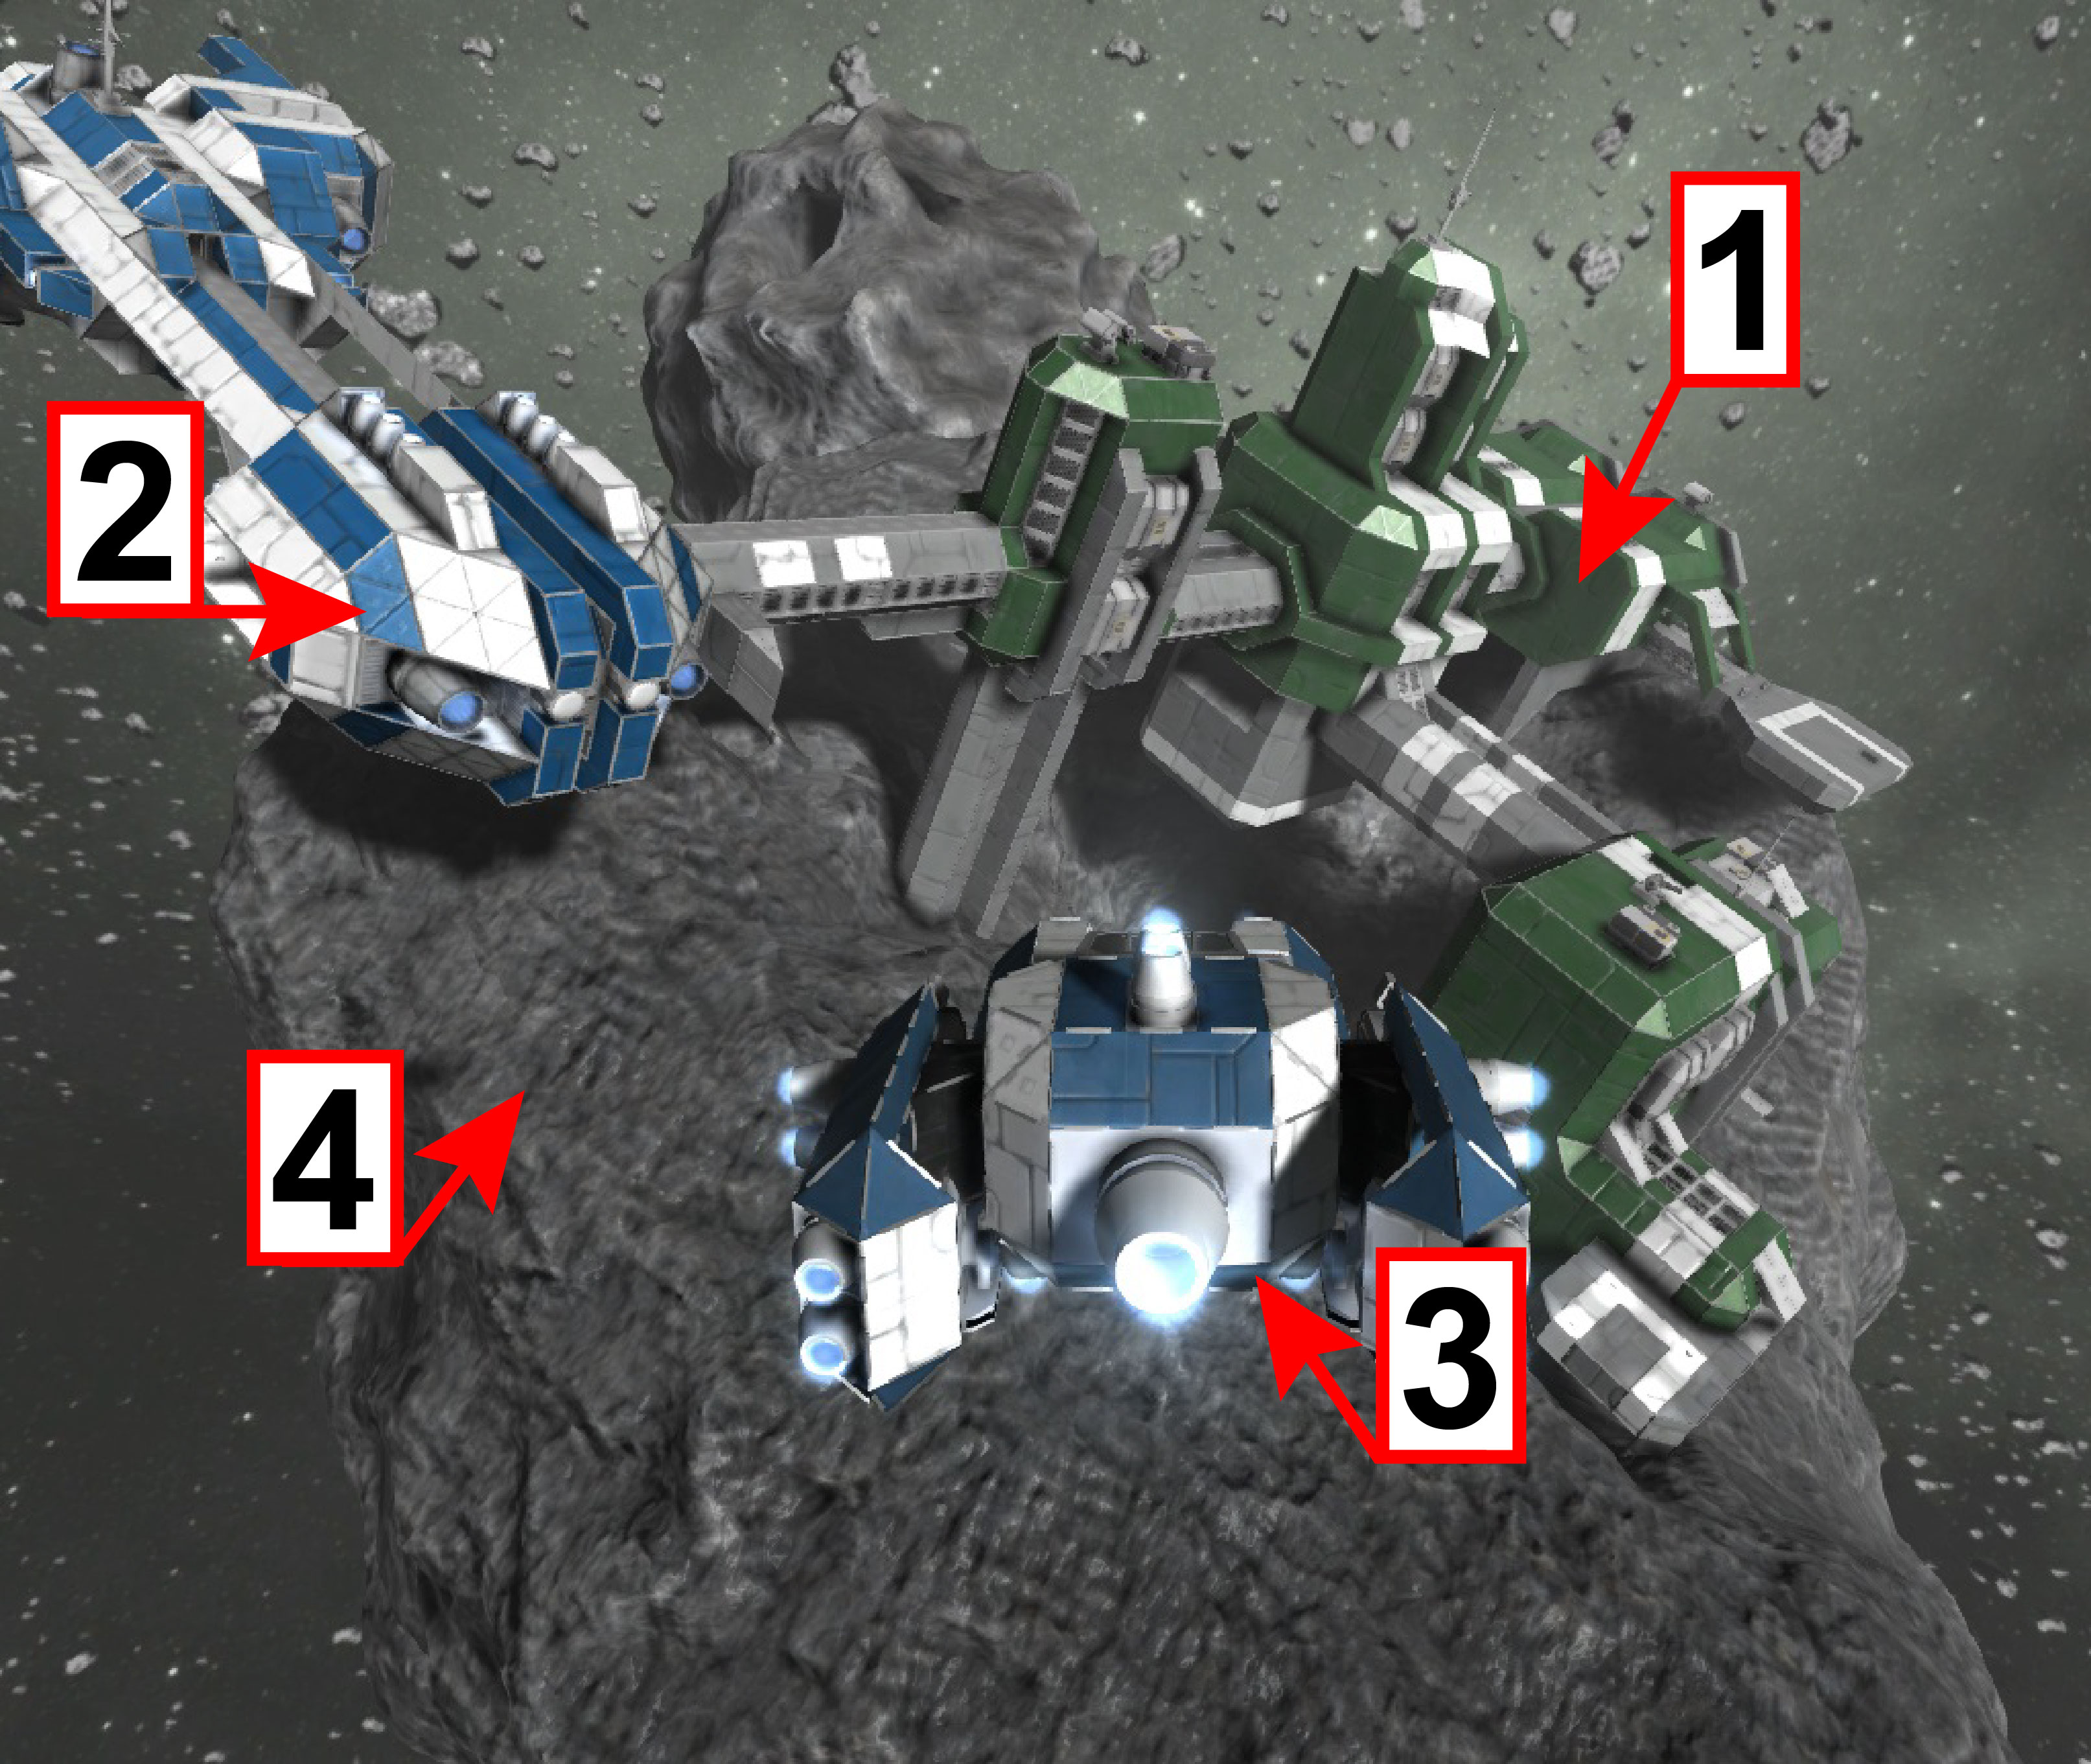
\includegraphics[ width=140mm]{../img/intro/se}

\caption{Hra Space Engineers - základna na asteroidu }
\label{fig:intro_se}

\end{figure}

\FloatBarrier


\subsection{Hry s maximálním důrazem na simulaci reality}

Do této sekce bychom měli zařadit například vesmírný simulátor \TM{}. // TODO popis, obrázek

bloky na stavění, ale třeba vozidla kompletní

\subsection{Ostatní - zařadit TODO }

Můžeme však nalézt i další příklady her (// TODO \TM{}, \NI{}, \PN{}, \ARK{}, \NMS{}).


\section{Herní bloky}



Obvykle je ve hře definován jeden základní rozměr bloku, který je neměnný. (\SE{} definuje více velikostí -- ty však nelze vzájemně kombinovat). To však může být problémem, pokud se hráč rozhodne postavit v herním světě nějakou větší a komplexnější strukturu podle reálné či fiktivní předlohy. Pro příklad uveďme některé výtvory ze hry \MC{}:
\begin{itemize}
	\item King's landing z knih Píseň ledu a ohně
	\item Minas Tirith - hlavní město Gondoru z univerza J.R.R. Tolkiena
\end{itemize}

Autoři těchto výtvorů museli volit takové měřítko, aby byly výtvory dostatečně detailní, ale zároveň aby bylo možné výtvor postavit v nějakém rozumném čase. Obecně ale můžeme říct, že čím větších detailů chtěli autoři dosáhnout, tím větší musel celý výtvor být, ale za ceny toho, že velké plochy trvaly o to déle.


\subsection{Náš návrh úpravy}
Chtěli bychom dát hráči k dispozici možnost ovlivňovat velikost bloku. Tím by mohl rychleji stavět rozsáhlejší struktury a přitom se věnovat i drobným či estetickým detailům.

\section{Inventář}
Dalším společným prvkem tohoto druhu her je inventář bloků, které může hráč umístit do herního světa. Hráč přes celé herní okno vidí \gls{hud}\citep{hud_terminology}, ve kterém má zobrazenou kromě jiného nabídku bloků, které má na rychlé volbě, může je snadno zvolit a daný blok umístit do herního světa. Navíc hry mohou definovat skupiny bloků (\SE{}, \ME{}), mezi kterými hráč může přepínat a tím rychle kompletně změnit sadu rychlé nabídky. Vidíme však limitaci v tom, že hráč musí ručně spravovat tyto seznamy a jednotlivé bloky (či nástroje) umisťovat do příslušných pozic.

Rádi bychom navrhli jiný způsob správy těchto sad, aby hráč jednou definoval, jaké prvky chce mít v příslušných sadách. Při vytvoření nového bloku by pak nemusel ručně editovat sadu, ale automaticky by měl tento nový blok k dispozici.  // TODO aplikovat do hry - typy bloků jako tagy

\section{Herní nepřítel}
Protože samotné stavění bez nějakého cíle či překážky není úplně zábavné, musíme hráči připravit nějakou překážku, komplikaci, kterou musí překonávat. Zde neexistuje jednoznačné řešení --- to je závislé na celkovém prostředí hry, zamýšlené cílově skupině a mnoha dalších faktorech. Cílem našeho hráče bude přežít kyselé deště. Ty budou přicházet v náhodných intervalech a budou sloužit jako překážka v rozvoji hry. Zároveň to ale bude pro hráče nástroj, jak získávat prostředky pro ochranu před dalšími dešti a rozvoj svých staveb. 


\section{Cíle práce}
Tato práce by měla naplnit následující cíle:
\begin{itemize}
	\item Bloky
	\item Inventář
	\item TODO
\end{itemize}

\iffalse

\begin{code}
  foo->bar( ).
\end{code}

{\tt tt text} a pokračuji díl.


Když se podíváme na hry jako například Minecraft, Space Engineers (nebo její odnož Medieval Engineers) tak zjistíme, že hra od hráče vyžaduje nejen stavitelské a konstruktérské schopnosti, ale také taktické dovednosti, které hráči umožňují v daném světě přežít. Mnohdy hráč může využít nevšedních technik daných mechanikami dané hry. Příkladem budiž farma na golemy ve hře Minecraft, která využívá bloky lávy, které jsou drženy cedulemi\citep{minecraft_tut_farm}.

V současné době jsou velikosti bloků omezeny na konstantné velikost. Ve hře Minecraft je blok hranově omezen na 1m, hra Space Engineers bloky omezuje dle kategorií od 0.5\,\rm m do 2.5\,\rm m \citep{se_blocks_wiki}.
My bychom se v této práci chtěli zabývat myšlenkou proměnlivé velikosti stavitelných bloků. Hráči by tak mohli ovlivňovat detailnost svých výtvorů, aniž by to muselo mít nutně negativní vliv na dobu nutnou k postavení komplexního, ale zároveň detailního výtvoru. Tato myšlenka však přináší spoustu problémů k řešení, které se však v této práci snažíme vyřešit.

Aby hra byla nebyla pro hráče nudná, měla by také obsahovat nějakého nepřítele - tedy něco, co bude hráče nutit se zlepšovat, překonávat nástrahy a posouvat se dále. I tomuto elementu hry se v této práci budeme věnovat. Zároveň nám to nabízí nové možnosti, jak do hry dodat prvky strategických her. Aby to hráč neměl tak jednoduché, bude muset taktizovat, aby svého nepřítele porazil, nebo alespoň v dané chvíli neprohrál, byť za cenu nějakých ztrát. xxd


\fi
